\scanpage{10}

% ll. 1–6
\mspage{\textcircled{8}}
\uline{Épinglage}. Fixons un triangle $(\alpha_4,\beta_4,\gamma_4)\in\widetilde\Gamma$ ($\alpha_4\in E(u)^*,\beta_4\in E(v)^*,\gamma_4\in E(w)^*$). Alors $\Pi_{22}(P_u)$ s'identifie à $P_u-\{\pi_u(\alpha_4)\}$, de $=\dots$. Ordonnons $V^*$, donc les $P_u-\{\pi_u(\alpha_4)\}$ etc. Dans $\unsure{E_u(u)^*|E(u)^*}-\{\alpha_4\}$ sur $P_u-\{\pi_u(\alpha_4)\}$ il y a une section $\{\alpha_1,\alpha_2,\alpha_3\}$, définie par

% ll. 7–9
\diagram{\(\displaystyle
\mathrm I_0\left\{\begin{array}{lll}
\alpha_1,\alpha_2,\alpha_3\ (\text{et }\alpha_4)&\text{liés à }\beta_4&\text{; de }=\\
\beta_1\ \beta_2,\beta_3\ (\text{et }\beta_{\unsure{3|4}})&\rule{1.15cm}{.35pt}\quad\gamma_4&\\
\gamma_1\ \gamma_2\ \gamma_3\ (\text{et }\gamma_4)&\rule{1.15cm}{.35pt}\quad\alpha_4&
\end{array}\right.
\)}

% ll. 10–14
Ainsi, en termes d'un ordre total sur $J=V^*$ et d'un ordre total (ou \unsure{seulemt|seulement} un ordre circulaire) sur \deleted{\unsure{$\Delta$}}\,$I:\{u,v,w\}$, on a épinglé les 24 \inserted{$=2\times12=2\times(3\times4)$} él. de $S^*$ (\unsure{en plus} des $u,v,w$) par les $\alpha_i,\beta_i,\gamma_i$, $\alpha'_i=\sigma\alpha_i$, $\beta'_i=\sigma\beta_i$, $\gamma'_i=\sigma\gamma_i$.

% ll. 15–16
De (I) et lem 3, on déduit [0] $\alpha_i$ lié à $\alpha'_i$ / $\beta_i$ à $\beta'_i$ /, $\gamma_i$ à $\gamma'_i$.

% left linking I to I' and [0]
\figure{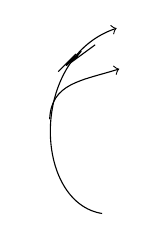
\begin{tikzpicture}[scale=.68]
\draw[->] (1,-2) .. controls (-.28,-1.8) and (-.38,.9) .. (1.27,1.46);
\draw[->] (.02,-.24) .. controls (.05,.44) and (.62,.48) .. (1.32,.70);
\draw (.18,.65)--(.51,.98)--(.33,.76)--(.61,1.03)--(.46,.85)--(.87,1.15);
\end{tikzpicture}}

% rows I prime
\diagram{\(\displaystyle
\mathrm I'\left\{\begin{array}{llll}
\alpha'_i\ \deleted{\unsure{\alpha_1,\alpha_2,\alpha_3}}&\text{liés à }\beta'_4,&\text{non à }\beta_4&\text{ni entre eux}\\
\beta'_i&\rule{.9cm}{.35pt}\quad\gamma'_4,&\text{non à }\gamma_4&\text{ni entre eux}\\
\gamma'_i&\rule{.9cm}{.35pt}\quad\alpha'_4,&\text{non à }\alpha_4&\text{ni entre eux}
\end{array}\right.
\)}

% rows I
\diagram{\(\displaystyle
\mathrm I\left\{\begin{array}{llll}
\alpha_i&\text{liés à }\beta_4,&\text{non à }\beta'_4&\text{ni entre eux}\\
\beta_i&\rule{1cm}{.35pt}\quad\gamma_4&\rule{.85cm}{.35pt}\quad\gamma'_4&\rule{1.4cm}{.35pt}\\
\gamma_i&\rule{1cm}{.35pt}\quad\alpha_4&\rule{.85cm}{.35pt}\quad\alpha'_4&\rule{1.4cm}{.35pt}
\end{array}\right.
\)}

% above rows II
\uline{Lemme} 8

% rows II
\diagram{\(\displaystyle
\mathrm{II}\left\{\begin{array}{lll}
\alpha_i\inserted{(1\leq i\leq3)}&\text{liés à }\gamma'_4,&\text{non à }\gamma_4\\
\beta_i&\rule{1cm}{.35pt}\quad\alpha'_4,&\rule{.9cm}{.35pt}\quad\alpha_4\\
\gamma_i&\rule{1cm}{.35pt}\quad\beta'_4,&\rule{.9cm}{.35pt}\quad\beta_4
\end{array}\right.
\)}

% rows II prime
\diagram{\(\displaystyle
\mathrm{II}'\left\{\begin{array}{lll}
\alpha'_i&\rule{1cm}{.35pt}\quad\gamma_4,&\text{non à }\gamma'_4\\
\beta'_i&\rule{1cm}{.35pt}\quad\alpha_4,&\rule{.9cm}{.35pt}\quad\alpha'_4\\
\gamma'_i&\rule{1cm}{.35pt}\quad\beta_4&\rule{.9cm}{.35pt}\quad\beta'_4
\end{array}\right.
\)}
% archive sheet number: 9
